\documentclass[10pt]{article}

\usepackage[utf8x]{inputenc}
\usepackage[T1]{fontenc}
\usepackage{amsfonts,amsmath,amssymb,amsthm,booktabs,color,graphicx}
\usepackage[ruled,vlined,linesnumbered]{algorithm2e}
\usepackage{enumitem}

\newtheorem{lemma}{Lemma}

\title{String Processing Algorithms 2015 - Week 2 Exercises}
\author{Rodion Efremov}
\date{\today}

\begin{document}
\maketitle

\section*{Exercise 1}
\color{blue} Outline algorithms that find the most frequent symbol in a give string.
\begin{enumerate}[label=(\alph*)]
\item for ordered alphabet, and
\item for integer alphabet.
\end{enumerate}
The algorithms should be as fast as possible. What are their (worst case) time complexities?  Consider also the case where $\sigma \gg n$. \color{black}

\subsection*{Solution}
\begin{algorithm}
\SetKw{KwLet}{let}
\SetKw{KwEmptyMap}{be an empty map}
\SetKw{KwNil}{nil}
\SetKw{KwNotMapped}{is not mapped in}
\KwLet $f$ \KwEmptyMap $f \colon \Sigma \to \mathbb{N}$ \\
$\mu = $ \KwNil \\
$L_{\mu} = 0$ \\
\For{$i = 1$ \KwTo $|S|$}{
	\If{$S[i]$ \KwNotMapped $f$}{
	    $f(S[i]) = 1$ \\
	    
	    \If{$L_{\mu} = 0$}{
	      $L_{\mu} = 1$ \\
	      $\mu = S[i]$ \\
	    }
	} \Else{
      $f(S[i]) = f(S[i]) + 1$ \\
      
      \If{$L_{\mu} < f(S[i])$}{
        $L_{\mu} = f(S[i])$ \\
        $\mu = S[i]$ \\
      }	
	}
}
\KwRet $\mu$ \\ 
\caption{\textsc{MostFrequentSymbol}$(S)$}
\end{algorithm}

\section*{Exercise 2}
\color{blue} Let $\mathcal{R} = \{ \texttt{manne}, \texttt{manu}, \texttt{minna}, \texttt{salla},\texttt{saul}, \texttt{sauli}, \texttt{vihtori} \}$.
\begin{enumerate}[label=(\alph*)]
\item Give the compact trie of $\mathcal{R}$.
\item Give the balanced compact ternary trie of $\mathcal{R}$.
\end{enumerate}
\color{black}

\subsection*{Solution}
\subsubsection*{(a)}
\begin{center}
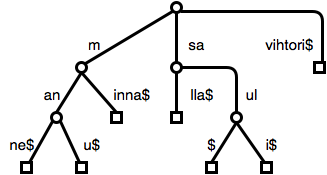
\includegraphics[scale=0.65]{CompactTrie}
\end{center}

\subsubsection*{(b)}
See the drawing.

\section*{Exercise 3}

\section*{Exercise 4}
\color{blue}
Prove
\begin{enumerate}[label=(\alph*)]
\item Lemma 1.14: For $i \in [2..n]$, $LCP_{\mathcal{R}}[i] = lcp(S_i, \{ S_1, \dots, S_{i - 1} \})$.
\item Lemma 1.15: $\Sigma LCP(\mathcal{R}) \leq \Sigma lcp(\mathcal{R}) \leq 2 \cdot \Sigma LCP(\mathcal{R})$.
\end{enumerate}
\color{black}
\subsection*{Solution}
Both by induction.

\subsubsection*{(a)}
We need an auxiliary lemma first: 
\begin{lemma}[Distance lemma]
If $S_1 < S_2 < S_3$, $lcp(S_1, S_3) \leq lcp(S_2, S_3)$.
\end{lemma}
\begin{proof}
The proof is by contradiction: Let $\text{prefix}(A, B)$ be the longest common prefix of $A$ and $B$. Assume that $l_1 > l_2$, where $l_1 = |\text{prefix}(S_1, S_3)|$ and $l_2 = |\text{prefix}(S_2, S_3)|$. Now $S_1 = a_1 a_2 \dots a_{l_2} \dots a_{l_1} b_1 b_2 \dots$ and $S_2 = a_1 a_2 \dots a_{l_2} b'_1 b'_2 \dots$. Because $S_3 = a_1 a_2 \dots a_{l_2} \dots a_{l_3} c_1 c_2 \dots$, we must have that $S_2 < S_1 < S_3$, which is a contradiction.
\end{proof}
Example
\begin{align*}
S_1: & aaaab \\
S_2: & aaaba \\
S_3: & aaabc
\end{align*}
\noindent \textbf{Base step}: Assume $i = 2$. Now $LCP_{\mathcal{R}}[2] = lcp(S_2, S_1) = lcp(S_2, \{ S_1 \})$. \\
\textbf{Induction step}: Assume that $LCP_{\mathcal{R}}[i] = lcp(S_i, \{ S_1, \dots, S_{i - 1} \})$. Now
\begin{align*}
lcp(S_{i + 1}, \{ S_1, \dots, S_i \}) &= \max \{ lcp(S_{i + 1}, S_i), lcp(S_{i + 1}, \{ S_1, \dots, S_{i - 1} \}) \} \\
											  		 &\overset{Dl}{=} lcp(S_{i + 1}, S_i),
\end{align*}
which concludes the proof.

\end{document}